\section{Prior Work}\label{sec:lit}
\subsection{Women in IT}\label{sec:lit-gender}
Modern computing is overwhelmingly male, according to a long, robust, and surprisingly consistent literature on gender in technology. \citet{Sanders2005Gender} summarizes research from the 1980s through the mid-2000s to show that women and girls regularly have less exposure to computers, especially programming; that they are less confident in their own computer skills, despite often being more proficient than their male peers; and that they are uncomfortable and uninterested in stereotypically macho tech culture.

Recent research focuses on the educational and professional consequences of those attitudes. Fewer women than men study computer science, and more women switch majors or drop out of the program \citep{Cohoon2006Just}. Similarly, fewer women enter careers in computing \citep{BartolAspray2006Transition}, and they change careers or leave the workforce at much higher rates than women in any other career path \citep{GlassEtAl2013Whats}. Most researchers see a causal relationship between women's low participation in computer science education and their low rates of employment in tech: fewer women study computer science, so fewer women find and keep computer science jobs. These studies employ the metaphor of a ``leaky pipeline'' \citep{Camp1997Incredible} and suggest that recruiting girls to computer science earlier in their education is the key to diversifying the IT workforce. More recent analyses, however, highlight the many different career paths that lead to IT work, arguing that a focus on the pipeline unduly ignores these alternate paths. Both perspectives agree that the lack of women in IT is a problem both for women and for IT as a field; the following sections summarize the two views.

\subsubsection{The Leaky Pipeline}
In the pipeline view, women are underrepresented in technical fields because they are neither encouraged to enter them nor given the support they need to remain. Studies investigating the leaky pipeline typically explore why girls never develop a serious interest in computer science \citep{BarkerEtAl2006Recruiting}, why female computer science majors frequently change departments \citep{KatzEtAl2006Traversing}, or specific techniques to improve female student retention (for instance, see the large literature on pair programming, e.g., \citealp{WernerEtAl2005Want, PorterEtAl2013Success}).

Gendered patterns in computer use appear well before high school: middle school boys are more likely to use computers for gaming, while girls use computers primary to communicate \citep{BarkerAspray2006State}. Increased exposure is correlated with greater confidence and interest in computers, so boys, with more varied computer experience, typically have much higher confidence in their own skills \citep{FrantomEtAl2002Measure}. Both gaps, in experience and in confidence, only widen as children get older \citep{FitzpatrickHardman2000Mediated}. These patterns have been documented since home computers were fairly uncommon \citep{JonesClarke1995Diversity}, but to my knowledge have not been investigated since the advent of ubiquitous mobile computing.

Formal computing education is also predominantly male, with fewer women than men studying information technology even as other STEM fields move toward gender parity. In 2004, just 16\% of high schoolers who took the Advanced Placement (AP) computer science exam were female; Physics B, the next-most disparate AP exam, had more than twice as many female test-takers at 34\% \citep{BarkerAspray2006State}. In a national study of computer science departments, \citet{Cohoon2006Just} found that women made up 24\% of undergraduate computer science majors, but comprised 32\% of the computer science students who switched to another major. Programs with higher female enrollment saw less-gendered attrition rates, corresponding with higher overall graduation rates and a more collaborative culture seen in departments that actively recruit and mentor female students \citep{MargolisFisher2002Unlocking}.

\subsubsection{Problems with the Pipeline Metaphor}
Unlike work on IT education, research on women in IT careers often rejects the notion of a pipeline and highlights instead the many possible paths to a career in technology. \citet{BartolAspray2006Transition} argue that the distinction between education and career implicit in the pipeline metaphor is rarely valid for knowledge workers, and note that jobs in IT are being created and filled much faster than traditional students are earning IT degrees. Many workers are entering IT from other pathways rather than from a computer science degree program. Women in particular are more likely to transition into tech from another field, whether by taking on more technical tasks within an existing role \citep{vonHellensEtAl2001Breaking}, by returning to school after some time in another career \citep{Jesse2006Poverty}, or by receiving vocational tech training \citep{Chapple2006Foot}.

\subsection{Narrative Data Visualization}\label{sec:lit-vis}
%% TODO:  Add Minard's Map %%
The most memorable data visualizations do not simply present data; they tell stories. Most iconically, Charles Minard's famous map, pictured in \autoref{fig:minard}, evocatively depicts Napoleon's Russian campaign of 1812 by mapping the army's journey and its size as 422,000 soldiers set out confidently, just 100,000 reach Moscow, and only a tenth of those make it home through the frigid winter weather. Many modern analysts, designers, journalists also use data to tell their stories. Established news sources like the \href{http://www.nytimes.com/interactive/2015/us/year-in-interactive-storytelling.html}{New York Times} and the \href{http://www.bbc.com/news/11628973}{BBC} feature interactive, data-driven stories, as do dedicated data journalism outlets like \href{http://fivethirtyeight.com/}{FiveThirtyEight}. Even personal correspondence can contain data stories, as with Giorgia Lupi and Stefanie Posavec's Dear Data project \citep{DearData}: the two sent each other weekly postcards visualizing an aspect of their lives that week, from the doors they opened in week 24 to the times they said goodbye in week 52. When they shared their project online, so many people connected with their data stories that their website now hosts mailing groups for other would-be data diarists.

\begin{figure}
  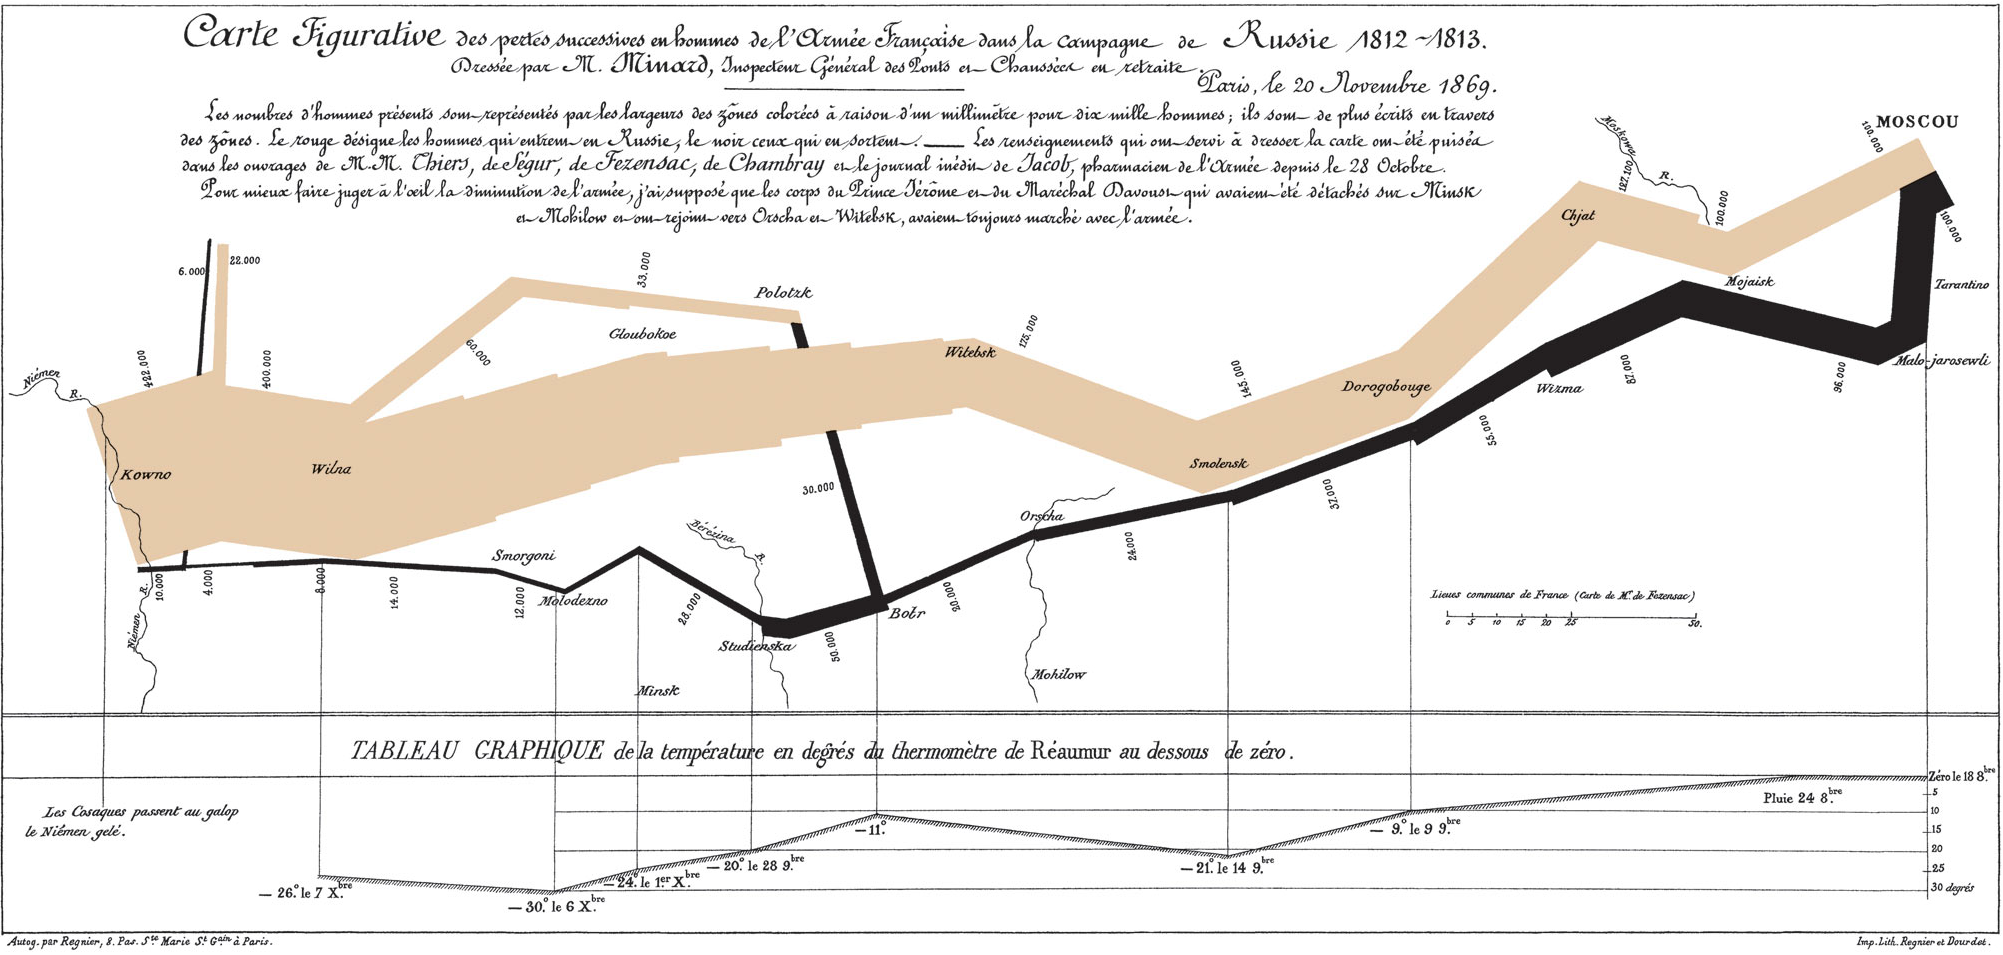
\includegraphics[width=\textwidth]{Minard}
  \caption{Charles Minard's Famous Map of Napoleon's Russian Campaign}
  \label{fig:minard}
\end{figure}

Narrative visualizations combine the engagement of storytelling with the authority of data analysis, creating a distinct medium that blends the author's message with the viewer's interactions. Not all visualizations either seek or achieve this balance, as \citet{LeeEtAl2015More} note; many visualizations are analytical tools that deliberately avoid narrative framing. But many visualizations are carefully crafted to illustrate the author's point. \citet{SegelHeer2010Narrative} identify four narrative structures commonly used to balance narrative and exploration in data stories: the checklist, which lets users explore a labeled storyboard of the interactive story; the interactive slideshow, which follows a traditional slideshow format but allows users to explore the data found on each slide; the drill-down story, which presents a summary graphic that illustrates the theme and lets users explore the underlying data; and the martini glass, which guides users through a tightly structured narrative before opening up into free exploration.

\subsubsection{Visual Narratives as Activism}
The combination of compelling story and convincing data makes visual narratives a natural tool for social or policy change. As early as the 1850s, John Snow, one of the fathers of modern epidemiology, used an annotated map to convince London officials to close a cholera-contaminated well \citep{Johnson2006Ghost}. In the same spirit, \citet{MichiganPublicRadio2016MAP} published an interactive map of lead levels in 4,000 households in Flint, MI to demonstrate that the problem affected the entire city.

Persuasive narrative visualization can also provide narrative framing to connect personal decisions and attitudes to larger issues. \citet{PandeyEtAl2014Persuasive} presented audiences with graphs or numerical statistics about a range of social issues; among viewers without strong prior opinions, significantly more were convinced by the simple graphics than by the numbers alone. However, \citet{KimEtAl2010Designing} demonstrate that visualizations without context---that is, visualizations that are not part of a narrative---do not show the same persuasive effects. They used graphical displays to encourage users to conserve energy by turning off their computers when not in use. One group saw a display of the time their computers sat idle, with no mention of energy conservation; the other saw an animation of a coral reef that got healthier as they reduced idle time. Although the coral visualization did not directly display their usage data, participants found it far more compelling than the standard idle tracker because it told a story by connecting their actions to environmental change.

With proper framing, simple visualizations can provide this narrative context as well as iconic representations like the coral reef. \citet{ZuckermanGalOz2014Deconstructing} evaluate the effectiveness of two different step trackers, one that includes a game and one that simply displays the user's daily steps as a bar chart filling toward their step goal. Their bar chart is visually quite similar to Kim et al's ineffective idle time tracker, and yet it was just as effective as the game in motivating participants to walk more. The bar chart in Zuckerman and Gal-Oz's study represents progress toward the user's own goals; it represents a simple but compelling narrative that motivates users to act.
